\chapter{Background} \label{sec:methods}
\section{Skinned Multi-Person Linear Model (SMPL)}
\begin{figure}[h]
    \centering
    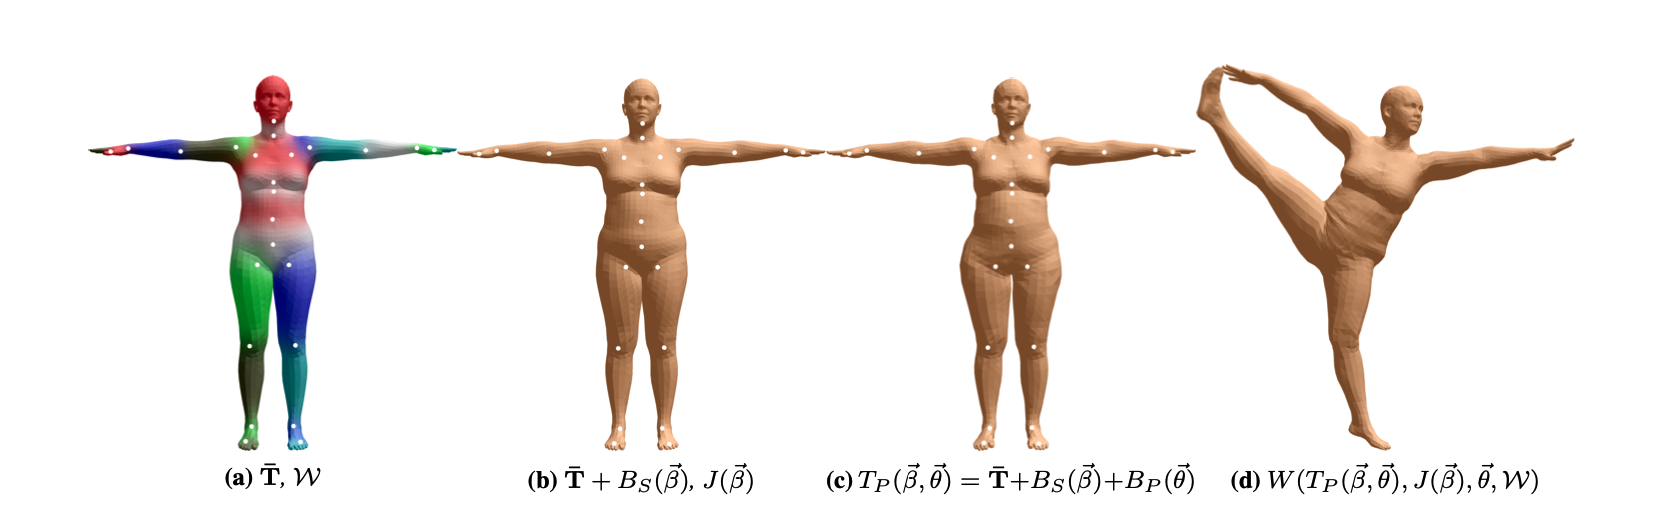
\includegraphics[width=\linewidth]{figures/smpl.png}
    \caption{SMPL model}
\end{figure}
The Skinned Multi-Person Linear (SMPL) model is a parametric body shape model that accurately represents a wide range of human bodies and poses. It is built upon a foundation of linear blend skinning enhanced with corrective blend shapes, which are derived from a large dataset of body scans. The model captures the subtle deformations that occur with different body shapes and poses and can easily be rendered due to its compatibility with existing graphics pipelines. Since its publication, several extensions such as DMPL, incorporating dynamic soft-tissue deformation and SMPL-X, also modelling hands and facial expressions have been introduced. The model is parameterized by $\vec{\beta}$, capturing the variations from a mean body shape and $\vec{\theta}$, specifying the axis-angle rotation of 23 of the template skeleton joints. Mathematically, the model can be expressed as:
\begin{equation}
    M(\vec{\beta}, \vec{\theta}) = W(T_P(\vec{\beta}, \vec{\theta}), J(\vec{\beta}), \vec{\theta}, \mathcal{W})
\end{equation}
where $T_P(\vec{\beta}, \vec{\theta})$ returns the vertices of the rest pose, incorporating the deformations from the body shape and pose and is given by:
\begin{equation}
    T_P(\vec{\beta}, \vec{\theta}) = \vect{\bar{T}} + B_S(\vec{\beta}) + B_P(\vec{\theta})
\end{equation}
$J(\vec{\beta})$ returns the 3D joint locations from the shaped template vertices using a learned regression matrix $\mathcal{J}$ and is given by:
\begin{equation}
    J(\vec{\beta}) = \mathcal{J}(\vect{\bar{T}} + B_S(\vec{\beta}))
\end{equation}
$W$ is the skinning function (e.g. Linear Blend Skinning (LBS) or Dual-Quaternion Blend Skinning (DQBS)) and $\mathcal{W}$ is the blend weights. 

\section{Human Mesh Reconstruction (HMR)}
Recovering the mesh of humans have several applications\dots

\section{Denoising Diffusion Probabilistic Models (DDPM)}
\begin{figure}[H]
    \centering
    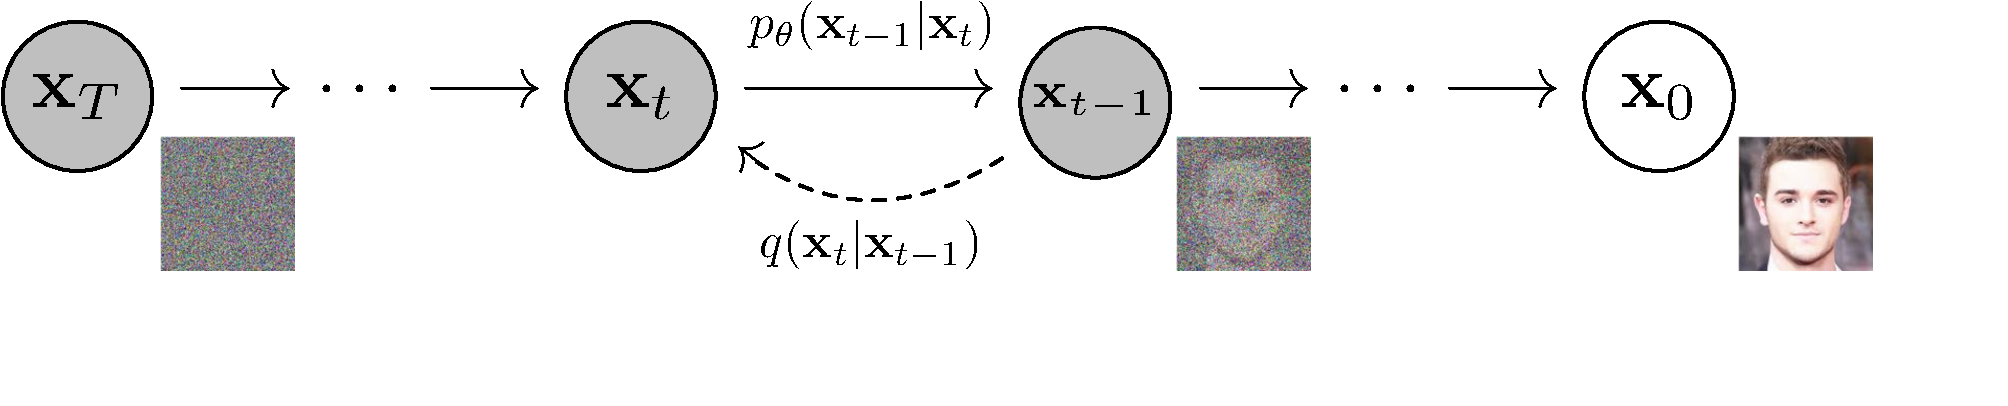
\includegraphics[width=\linewidth]{figures/pgm_diagram_xarrow_small.pdf}
    \caption{Diffusion forward and backward process (taken from \cite{ho2020denoising})}
    \label{fig:diffusion-process}
\end{figure}
In recent years, several types of generative models such as Variational Autoencoders (VAEs), Generative Adverserial Networks (GANs), autoregressive models and flow-based models have shown remarkable results in data generation of varying data modalities, such as images, audio, videos and text. Most recently, Denoising Diffusion Probabilistic Models (DDPMs) have gained large popularity especially within the field of image generation due to several reasons such as high-quality data generation, versitility in several data domains as well as controllability, allowing one to steer the generation towards desired outputs.

A DDPM is a parametarized Markov chain trained using variational inference to reverse a (forward) diffusion process, $q(\vect{x}_{1:T} \mid \vect{x}_0)$, as seen in \cref{fig:diffusion-process} wherein the signal of the data, $\vect{x}_0$, is gradually destroyed by adding gaussian noise according to predefined noise schedule $\{\beta_t  \in (0,1) \}_{t=1}^T$ giving rise to increasingly noisy samples, $\vect{x}_1 \ldots \vect{x}_T$. 

The forward process is defined as follows:
\begin{equation}    
    q(\vect{x}_{1:T} \mid \vect{x}_{0}) = \prod_{t=1}^T q(\vect{x}_{t} \mid \vect{x}_{t-1}), \quad q(\vect{x}_{t} \mid \vect{x}_{t-1}) = \mathcal{N}(x_{t}; \sqrt{1 - \beta_t}\vect{x}_t,\beta_t \vect{I} )
\end{equation}
with $T$ being the discritized number of diffusion steps before all original information is completely discarded. The goal of the inverse or backwards process then becomes to iteratively remove the noise, in order to arrivate at the original data. More formally, the process is defined as:
\begin{equation}
    p_\theta(\vect{x}_{0:T}) = p(\vect{x}_T) \prod_{t=1}^T p_\theta(\vect{x}_{t-1} \mid x_{t}), \quad p_\theta(\vect{x}_{t-1} \mid \vect{x}_{t}) = \mathcal{N}\left(\vect{x}_{t-1}; \vect{\mu}_\theta(\vect{x}_t, t), \vect{\Sigma}_\theta(\vect{x}_t, t) \right)
\end{equation}
taking starting point in pure noise $p(\vect{x}_T) = \mathcal{N}(\vect{x}_T; \vect{0}, \vect{I})$, incrementally removing the noise through the learned functions, $\vect{\mu}_\theta(\vect{x}_t, t)$ and $\vect{\Sigma}_\theta(\vect{x}_t, t)$ commonly parameterized by a deep neural network.
Using the reparameterization trick, we are able to sample any noisy version of our data, $\vect{x}_t$, at time step $t$ given our original data $\vect{x}_0$. Recall our forward transition probability function, $q(\vect{x}_t \mid \vect{x}_{t-1})$. Letting $\alpha_t = 1 - \beta_t$, $\bar{\alpha}_t = \prod_{i=1}^t \alpha_i$ and using the reparameterization trick the expression can be rewritten as:
\begin{equation}
    \vect{x}_t = \sqrt{\alpha_t} \vect{x}_{t-1} + \sqrt{1 - \alpha_t} \epsilon_{t-1}
\end{equation}
where $\epsilon_{t-1} \sim \mathcal{N}(0,1)$. Expanding the recursive definition then gives:
\begin{align*}
    \vect{x}_t    % & = \sqrt{\alpha_t} \vect{x}_{t-1} + \sqrt{1 - \alpha_t} \vect{\epsilon_{t-1}} \\
                    & = \sqrt{\alpha_t} \left( \sqrt{\alpha_{t-1}} \vect{x}_{t-2} + \sqrt{1 - \alpha_{t-1}} \vect{\epsilon}_{t-2} \right) + \sqrt{1 - \alpha_t} \vect{\epsilon_{t-1}} \\
                    % & = \sqrt{\alpha_t \alpha_{t-1}} \vect{x}_{t-2} + \sqrt{\alpha_t(1 - \alpha_{t-1})} \vect{\epsilon_{t-2}} + \sqrt{1 - \alpha_{t}} \vect{\epsilon_{t-1}} \\
                    & = \sqrt{\alpha_t \alpha_{t-1}} \vect{x}_{t-2} + \sqrt{1 - \alpha_{t}\alpha_{t-1}} \vect{\bar{\epsilon}}_{t-2}
\end{align*}
where $\vect{\bar{\epsilon}}_{t-2}$ merges the two independent Gaussians $\vect{\epsilon}_{t-1}$ and $\vect{\epsilon}_{t-2}$ into a single Gaussian with new variance as the sum of variances $\alpha_t (1 - \alpha_{t-1}) + (1 - \alpha_{t}) = 1 - \alpha_t \alpha_{t-1}$. Recursively applying the definition of $\vect{x}_t$ and merging the gaussian noise terms results in the simplified expression:
\begin{equation} \label{eq:nice}
    \vect{x}_t = \sqrt{\bar{\alpha}_t}\vect{x}_0 + \sqrt{1 - \bar{\alpha}_t} \vect{\epsilon}, \quad \vect{\epsilon} \sim \mathcal{N}(\vect{0}, \vect{I})
\end{equation}
% or by undoing the reparameterization:
% \begin{equation}
%     q(\vect{x}_t \vert \vect{x}_0) = \mathcal{N}(\vect{x}_t; \sqrt{\bar{\alpha}_t} \vect{x}_0, (1 - \bar{\alpha}_t)\vect{I})
% \end{equation}
%This result enables sampling of any noisy version of $\vect{x}_t$ at time $t$ given "clean" data $\vect{x}_0$. 
Conversely, given $\vect{x}_0$, the reverse conditional probability:
\begin{equation*}
    q(\vect{x}_{t-1} \vert \vect{x}_t, \vect{x}_0) = \mathcal{N}\left( \vect{x}_{t-1}; \vect{\tilde{\mu}}_t(\vect{x}_t, \vect{x}_0), \tilde{\beta}_t \vect{I} \right)
\end{equation*}
becomes tractable to compute using Bayes rule (derivation in \cref{appendix:q-posterior-derivation}) with mean and variance given by:
\begin{align} \label{eq:x-t-min-1-from-x-t}
    \vect{\tilde{\mu}}_t(\vect{x}_t, \vect{x}_0) &= \frac{\sqrt{\bar{\alpha}_{t-1}} \beta_t}{1-\bar{\alpha}_t} \vect{x}_0+\frac{\sqrt{\alpha_t}\left(1-\bar{\alpha}_{t-1}\right)}{1-\bar{\alpha}_t} \vect{x}_t \overset{\text{Using \ref{eq:nice}}}{=} \frac{1}{\sqrt{\alpha_t}}\left(\vect{x}_t-\frac{1-\alpha_t}{\sqrt{1-\bar{\alpha}_t}} \vect{\epsilon}_t\right) \\
    \tilde{\beta}_t &= \frac{1-\bar{\alpha}_{t-1}}{1-\bar{\alpha}_t} \beta_t
\end{align}
The model is trained by optimizing the variational lower bound on the log likelihood:
\begin{equation}
    L_{VLB}
        = \mathbb{E}_q\left[ \log \frac{p_\theta(\vect{x}_{0:T})}{q(\vect{x}_{1:T} \vert \vect{x}_0)}\right]
        = \mathbb{E}_q\left[\log p(\vect{x_T}) + \sum_{t \geq 1} \log \frac{p_\theta(\vect{x}_{t-1} \vert \vect{x}_{t})}{q(\vect{x}_t \vert \vect{x}_{t-1})}
        \right]
        \leq \mathbb{E}\left[\log p_\theta(\vect{x}_0)\right]
\end{equation}
which in practice means minimizing the negative variational lower bound. 
\cite{ho2020denoising} rewrites this into a sum of KL-divergences:
\begin{equation}
    L_{VLB} = \mathbb{E}_q \left[ \underbrace{D_{\mathrm{KL}} \left(
            q\left(\vect{x}_T \mid \vect{x}_0\right) \| p\left(\vect{x}_T\right)
            \right)}_{L_T} + \sum_{t=2}^T \underbrace{D_{\mathrm{KL}}\left(q\left(\vect{x}_{t-1} \mid \vect{x}_t, \vect{x}_0\right) \| p_\theta\left(\vect{x}_{t-1} \mid \vect{x}_t\right)\right)}_{L_{t-1}} - \underbrace{\log p_\theta\left(\vect{x}_0 \mid \vect{x}_1\right)}_{L_0} \right]
\end{equation}
where the authors model $L_0$ from seperate discrete decoder. As $L_T$ doesn't depend on our parameters, $\theta$, and is therefore constant, it can be ignored during optimization. The rest of the $L_{t-1}$ terms can be efficiently computed in the closed form, by fixing the variance $\vect{\Sigma}_\theta(\vect{x}_t, t) = \sigma_t^2 \vect{I}$ to only depend on the current timestep (authors propose $\sigma_t^2 = \beta_t$ or $\sigma_t^2 = \tilde{\beta}_t$). $L_{t-1}$ can then be written in closed form (derivation in \cref{appendix:L-closed-form}) as:
\begin{equation}
    L_{t-1} = \mathbb{E}_q \left[ \frac{1}{2\sigma_t^2} \| \vect{\tilde{\mu}}_t(\vect{x}_t, \vect{x}_0) - \vect{\mu}_\theta(\vect{x}_t, t) \|^2 \right] + C_t
\end{equation}
where $C_t$ is a constant depending on the choice of $\sigma_t^2$ and the noise schedule. Using \cref{eq:x-t-min-1-from-x-t} \cite{ho2020denoising} reparameterize the expression in terms of predicting the noise:
\begin{equation}
    L_{t-1} = \mathbb{E}_{\vect{x}_0, \vect{\epsilon}}\left[
        \frac{\beta_t^2}{2 \sigma_t^2 \alpha_t \left( 1 - \bar{\alpha}_t\right)} \left\| 
            \vect{\epsilon}-\vect{\epsilon}_\theta \left(\sqrt{\bar{\alpha}_t} \vect{x}_0+\sqrt{1-\bar{\alpha}_t} \vect{\epsilon}, t\right)
            \right\|^2
    \right]
\end{equation}
as they find it leads to better unconditional sample quality when training on the CIFAR10 dataset. Furthermore, they report the best sample quality when using the "simple" objective, ignoring the weighing:
\begin{equation} \label{eq:ddpm-simple-objective}
    L_\mathrm{simple} = \mathbb{E}_{t \sim \mathcal{U}(1, T),\ \vect{\epsilon}} \left[
        \vect{\epsilon} - \vect{\epsilon}_\theta( \sqrt{\bar{\alpha}} \vect{x}_0 + \sqrt{1 - \bar{\alpha}}\vect{\epsilon}, t)
    \right]
\end{equation}

The final training and sampling scheme, as outlined in \cref{alg:training} and \cref{alg:sampling} can be summarized as follows. The training algorithm optimizes the model to predict and remove noise from data, while the sampling algorithm uses the trained model to iteratively transform random noise into structured data.

\algrenewcommand\algorithmicindent{0.5em}%
\begin{figure}[t]
\begin{minipage}[t]{0.495\textwidth}
\begin{algorithm}[H]
  \caption{Training} \label{alg:training}
  \small
  \begin{algorithmic}[1]
    \Repeat
      \State $\vect{x}_0 \sim q(\vect{x}_0)$
      \State $t \sim \mathrm{Uniform}(\{1, \dotsc, T\})$
      \State $\vect{\epsilon}\sim\mathcal{N}(\vect{0},\vect{I})$
      \State Take gradient descent step on
      \Statex $\qquad \grad_\theta \left\| \vect{\epsilon} - \vect{\epsilon}_\theta(\sqrt{\bar\alpha_t} \vect{x}_0 + \sqrt{1-\bar\alpha_t}\vect{\epsilon}, t) \right\|^2$
    \Until{converged}
  \end{algorithmic}
\end{algorithm}
\end{minipage}
\hfill
\begin{minipage}[t]{0.495\textwidth}
\begin{algorithm}[H]
  \caption{Sampling} \label{alg:sampling}
  \small
  \begin{algorithmic}[1]
    \vspace{.04in}
    \State $\vect{x}_T \sim \mathcal{N}(\vect{0}, \vect{I})$
    \For{$t=T, \dotsc, 1$}
      \State $\vect{z} \sim \mathcal{N}(\vect{0}, \vect{I})$ if $t > 1$, else $\vect{z} = \vect{0}$
      \State $\vect{x}_{t-1} = \frac{1}{\sqrt{\alpha_t}}\left( \vect{x}_t - \frac{1-\alpha_t}{\sqrt{1-\bar\alpha_t}} \vect{\epsilon}_\theta(\vect{x}_t, t) \right) + \sigma_t \vect{z}$
    \EndFor
    \State \textbf{return} $\vect{x}_0$
    \vspace{.04in}
  \end{algorithmic}
\end{algorithm}
\end{minipage}
\vspace{-1em}
\end{figure}

% To summarize, diffusion models are generative models that create data by reversing a diffusion process. They are trained using a simplified version of the variational lower bound on the log-likelihood. Starting from pure noise, the model iteratively removes the predicted noise through a step-by-step denoising process, effectively reconstructing the original data. This approach allows DDPMs to produce high-quality and diverse outputs.

\subsection{Variance schedules}
\begin{figure}[H]
    \centering
    \begin{subfigure}[b]{0.49\linewidth}
        \centering
        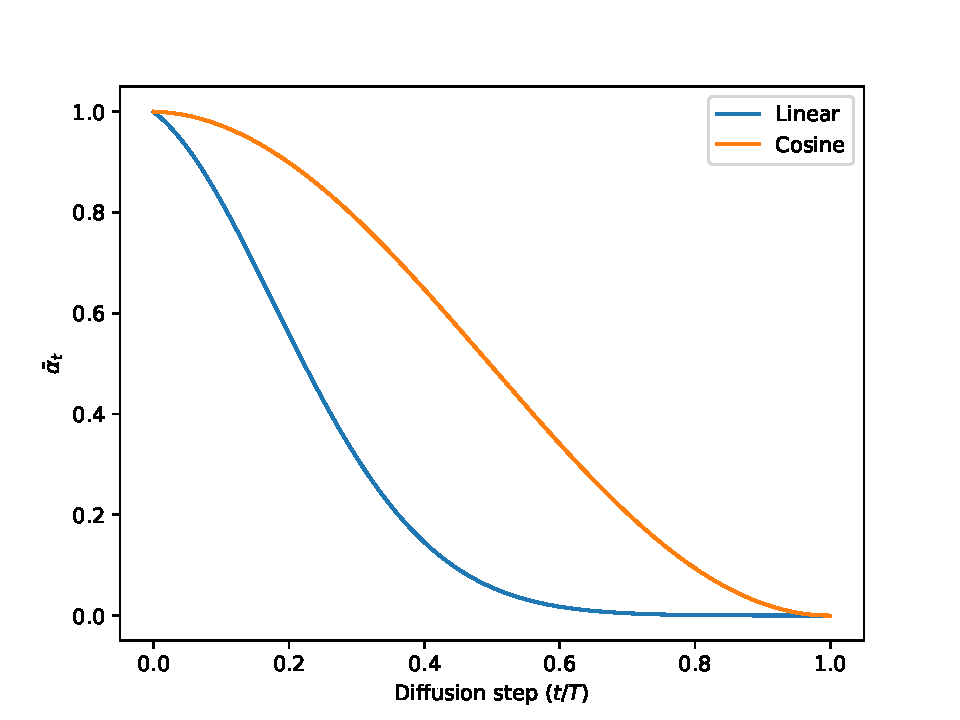
\includegraphics[width=\linewidth]{figures/schedule.pdf}    
    \end{subfigure}
    \hfill
    \begin{subfigure}[b]{0.49\linewidth}
        \centering
        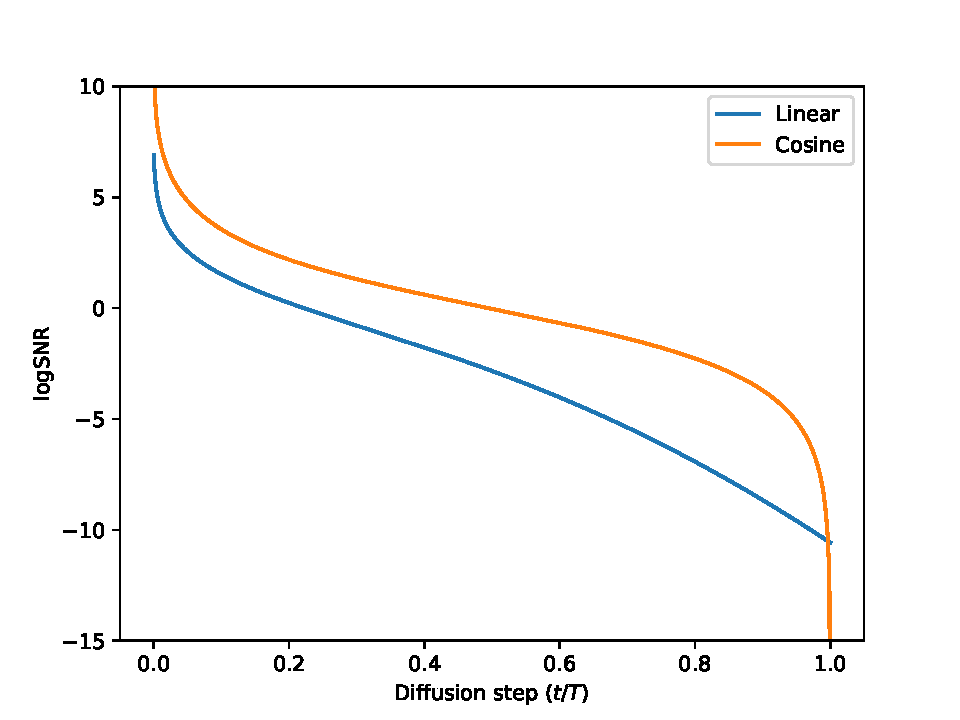
\includegraphics[width=\linewidth]{figures/snr.pdf}    
    \end{subfigure}
    \caption{Linear and cosine schedule and signal-to-noise ratio.}
    \label{fig:schedule}
\end{figure}
In the DDPM paper \cite{ho2020denoising} choose a variance schedule with $\beta_t$ linearly increasing from $\beta_1 = 10^{-4}$ to $\beta_T = 0.02$. However, this results in $\vect{x}_t$ almost entirely losing its signal in the last quarter of the schedule as problematized by \cite{pmlrv139nichol21a}. The authors instead propose a cosine variance schedule, where the squared signal proportion is given by:
\begin{equation}
    \bar{\alpha}_t=\frac{f(t)}{f(0)}, \quad f(t)=\cos \left(\frac{t / T+s}{1+s} \cdot \frac{\pi}{2}\right)^2
\end{equation}
where $s$ controls the offset of the noise schedule. The authors set $s=0.008$ as they found that $s=0$ resulted in minuscule noise near $t=0$ making it hard for the model to predict $\epsilon$. From $\bar{\alpha}_t$ one can then compute $\beta_t = \min\left( 1 - \frac{\bar{\alpha}_t}{\bar{\alpha}_{t-1}}, 0.999 \right)$ with the $\min$ to prevent singularities. A comparison of the cosine and linear schedules can be seen in \cref{fig:schedule}. 


\subsection{Classifier and Classifier-Free Guidance (CFG)}
% When sampling from generative models, one often wants to conditionally generate samples from the data distribution of different sub categories. One method for doing so with diffusion models is classifier guidance. Here the generation process relies on an external model guiding the reverse diffusion process towards the sub category date manifold. We first define the score-function as the gradient of the log-likelihood:
% \begin{equation}
%     s_\theta(\vect{x}) = \grad_{\vect{x}} \log p_\text{data}(\vect{x})
% \end{equation}

% \begin{equation}
%     \dot{\vect{x}} = 
% \end{equation}

% \begin{equation}
%     \grad_{\vect{x}_t} \log p_\theta\left(\vect{x}_t\right)=-\frac{1}{\sqrt{1-\bar{\alpha}_t}} \vect{\epsilon}_\theta\left(\vect{x}_t\right)
% \end{equation}

% \cite{dharial2021diffusion}
In practice, it is often desirable to steer the generation process in order to output data belonging to a specific class, such as cats or dogs in the context of image generation, or incorporating some other information relevant for the output. This process can be framed within the context of probability theory as conditional generation, where the aim is to maximize the probability of the data, $\vect{x}$, given some conditioning signal, $y$, (e.g. a class label. According to Bayes' rule, the conditional probability can be expressed as:
\begin{equation}
    p(\vect{x} \mid y) = \frac{p(\vect{x}, y)}{p(y)} \propto p(y \mid \vect{x}) p(\vect{x})
\end{equation}
Hence, it is proportional to the joint probability of the data and label, which from basic probability theory is equal to the product of the unconditional probability of the data, $p(\vect{x})$, and the probability of the conditioning signal given the data, $p(y \mid \vect{x})$ (for labels; that the data belonging to the given class). In the DDPM paper \cite{ho2020denoising} establishes connection between diffusion models and Noise-Conditioned Score Networks (NCSN) and shows how the reverse diffusion process can be seen as a temporal discritized type of annealed Langevin dynamics given by the stochastic differential equation:
\begin{equation}
    \frac{d}{dt} \log p(\vect{x}_t) = \sqrt{\bar{\alpha}_t} s(\vect{x}_t, t) + \sqrt{1 - \bar{\alpha}_t} \vect{z}_t
\end{equation}
where $z_t \sim \mathcal{N}(0, 1)$ and $s(\vect{x}_t, t) = \grad_{\vect{x}_t} \log p(\vect{x}_t)$ is referred to as the score function. It turns out that the denoising network can be used to approximate the score function:
\begin{equation}
    s(\vect{x}_t, t) \approx -\frac{1}{\sqrt{1 - \bar{\alpha}_t}} \vect{\epsilon}_\theta(\vect{x}_t, t)
\end{equation}
Returning to the factorization of the conditional probability, taking the gradient of the log of both sides reveals the relationship with the score function:
\begin{equation}
    \grad_{\vect{x}_t} \log p(\vect{x}_t \mid y ) = \grad_{\vect{x}_t} \log p(y \mid \vect{x}_t) + \underbrace{\grad_{\vect{x}_t} \log p(\vect{x}_t)}_{s(\vect{x}_t, t)}
\end{equation}
\cite{dharial2021diffusion} trains a classifier, $f_\phi(y \mid \vect{x}_t) \approx p(y \mid \vect{x}_t)$, seperately to predict the class label of noisy images. By using the reformulated denoising function:
\begin{equation}
    \bar{\vect{\epsilon}}_{\theta}(\vect{x}_t, t) = \vect{\epsilon}_\theta(\vect{x}_t, t) - \sqrt{1 - \bar{\alpha}_t} \grad_{\vect{x}_t} \log f_\phi(y \mid \vect{x}_t)
\end{equation}
where $s$ controls guidance strength, it is possible to guide the diffusion sampling e.g. in order to generate images of a specific category, hence the name classifier guidance. 



% Write about classifier-free guidance.
% 



\section{Tranformer architecture}
\begin{figure}[H]
    \centering
    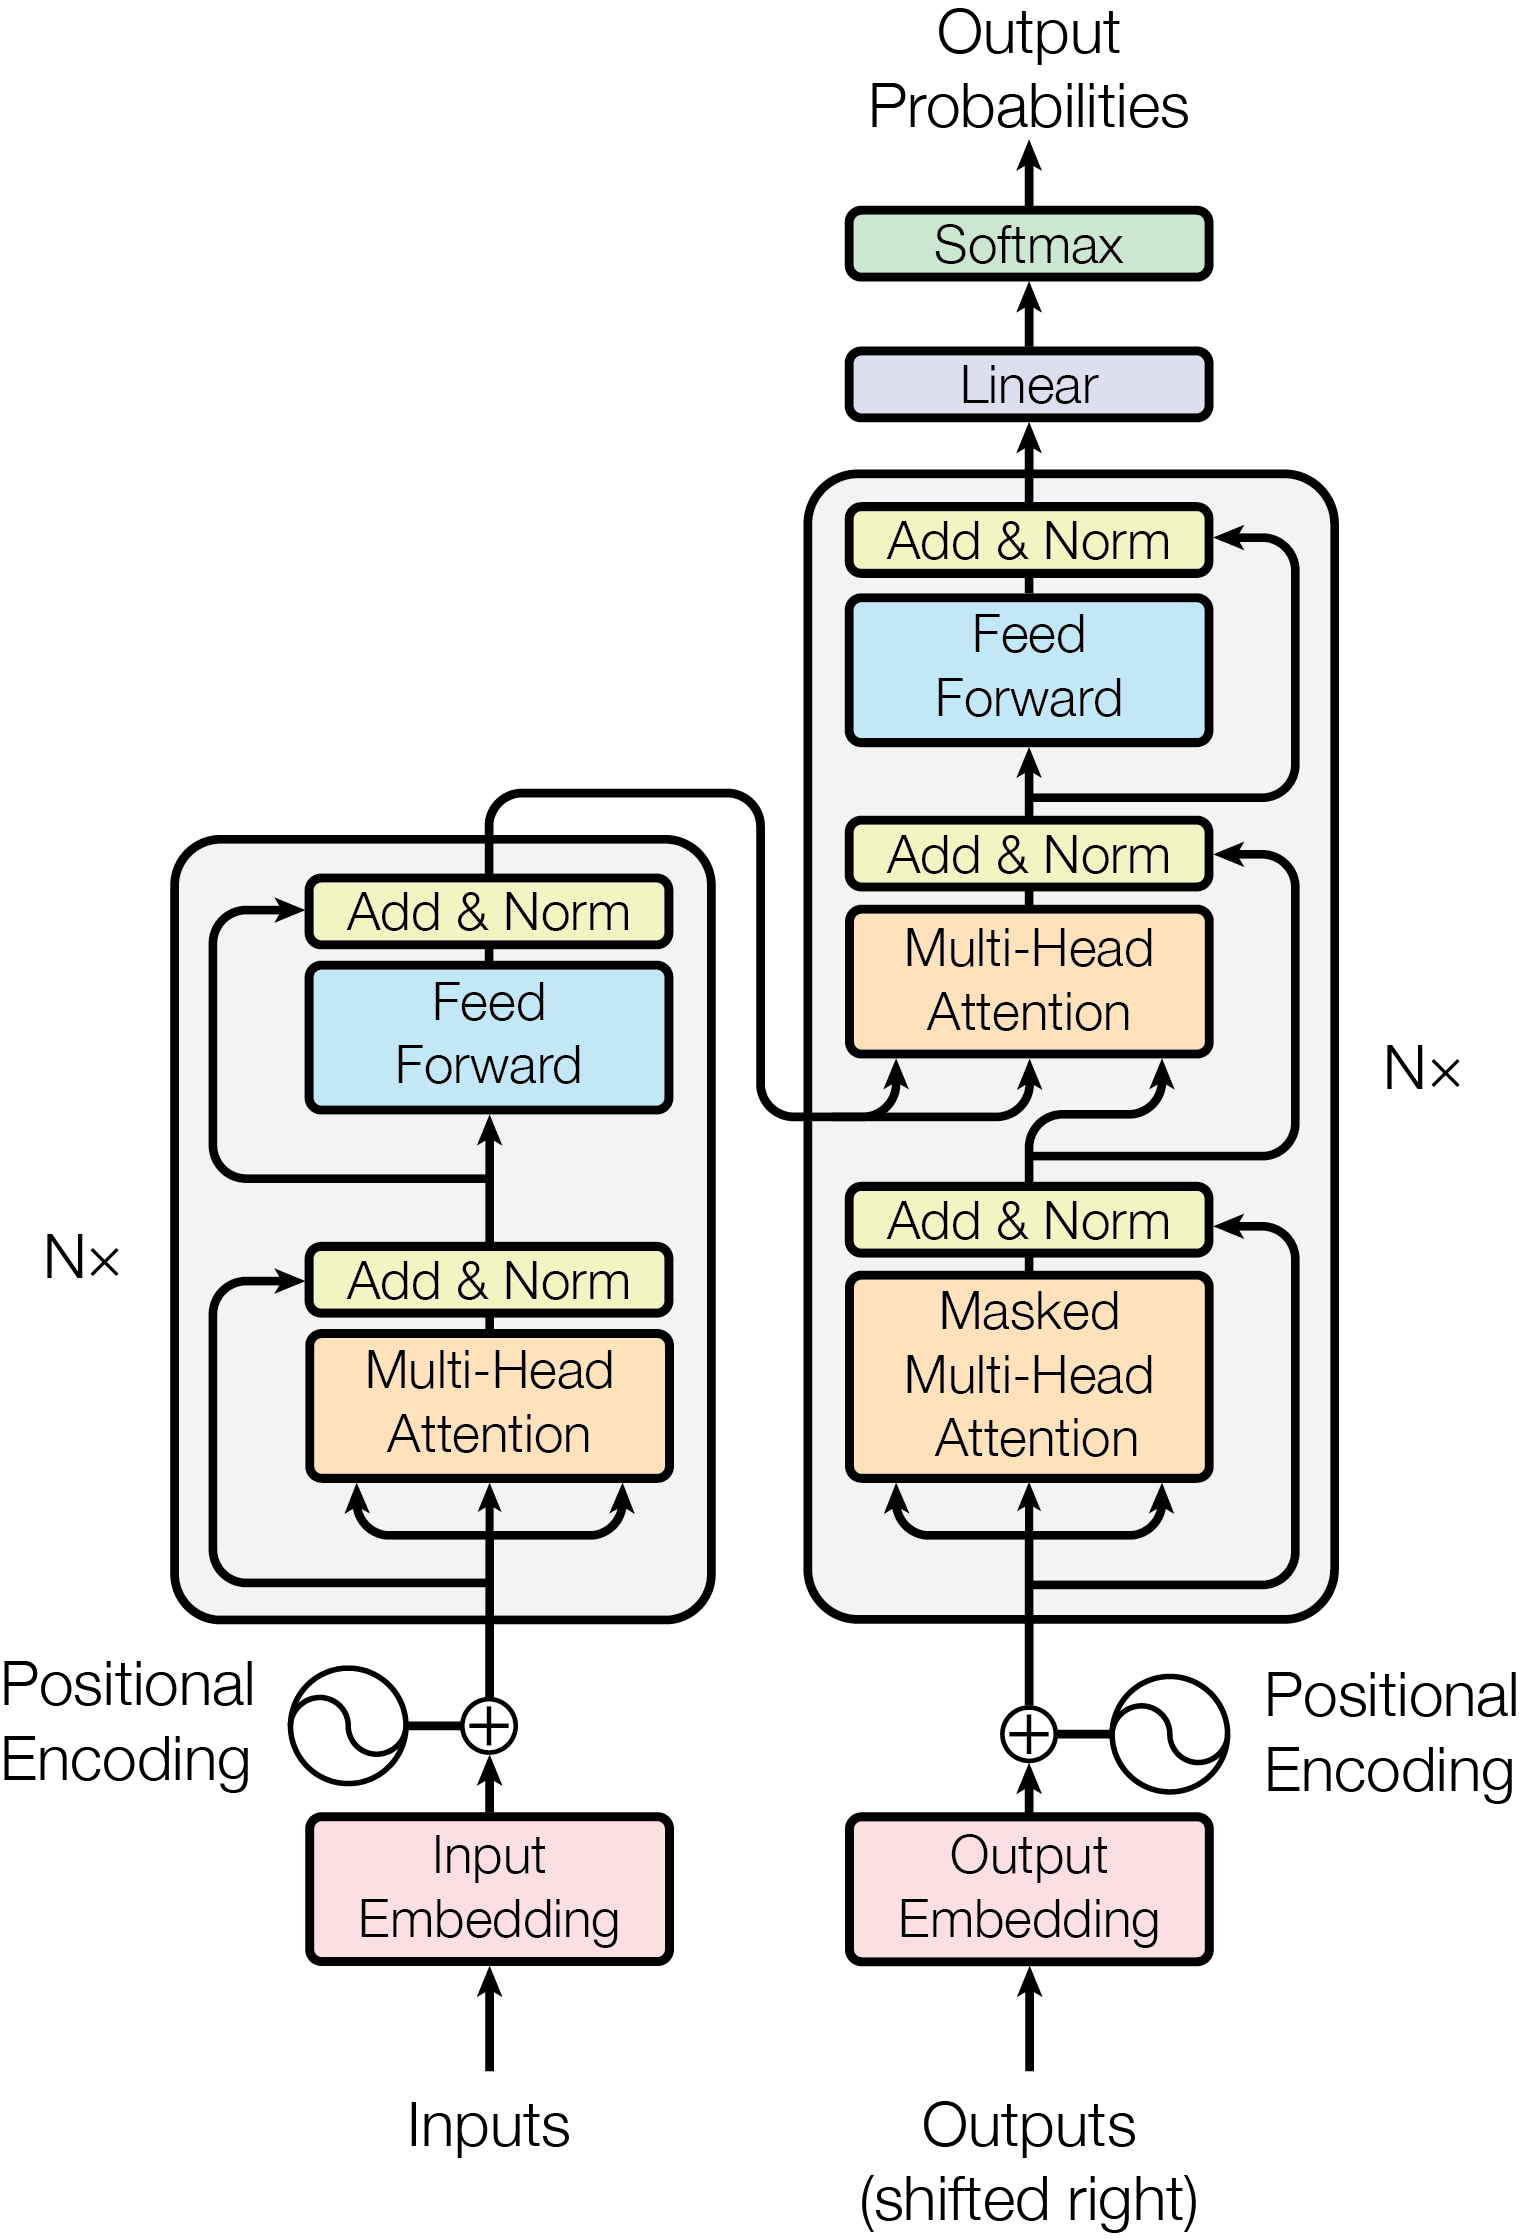
\includegraphics[width=0.4\linewidth]{figures/transformer.png}
    \caption{The transformer (Image from \cite{transformer2017}.)}
\end{figure}
The transformer model, introduced by \cite{transformer2017}, revolutionized natural language processing (NLP) and machine translation. This model was designed as an alternative to the traditional recurrent sequence models, such as the seq2seq model by \cite{seq2seq}, which had been widely used in NLP tasks.
\begin{figure}[H]
    \centering
    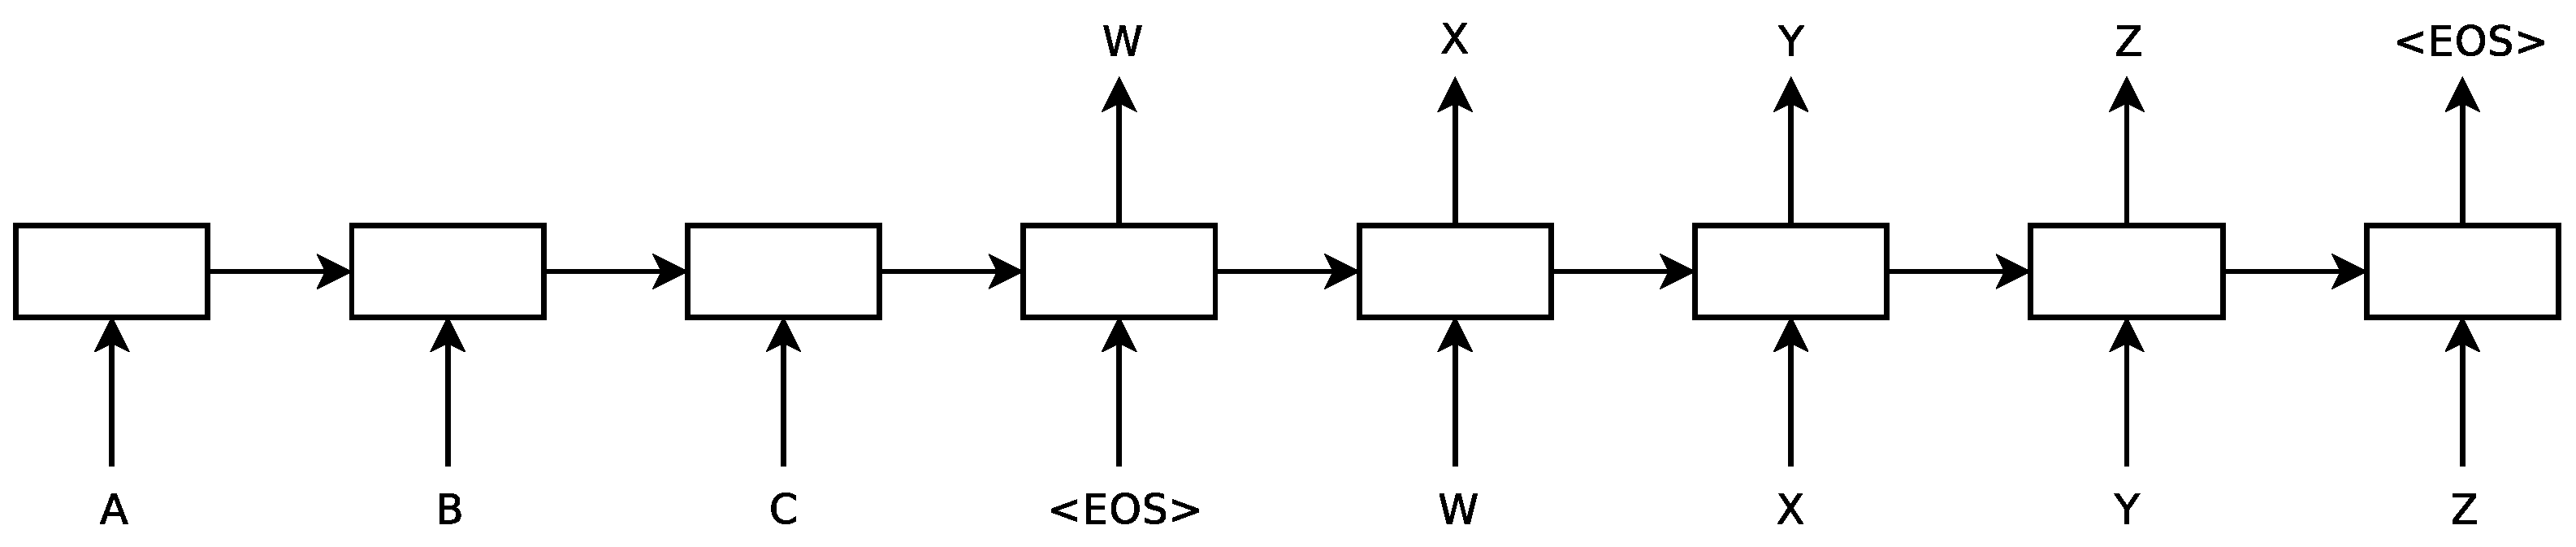
\includegraphics[width=0.8\linewidth]{figures/seq2seq.eps}
    \caption{The seq2seq model by \cite{seq2seq}.}
    \label{fig:seq2seq}
\end{figure}
The seq2seq model (as illustrated in \cref{fig:seq2seq}) encodes an input sequence into a context vector and then decodes the output sequence from this vector in a sequential manner. This approach often results in an information bottleneck, particularly when dealing with long-range dependencies within the data.

In contrast, the transformer model utilizes an attention mechanism, enabling more effective communication between tokens without relying on sequential processing of hidden states. The architecture comprises an encoder and a decoder. The encoder uses multi-headed self-attention to create semantic representations for each token in the input sequence, allowing the model to process the entire context simultaneously.

The decoder then uses these representations through cross-attention and causal self-attention mechanisms. Cross-attention integrates information from the encoder's output, while causal self-attention ensures that the model only considers previously generated tokens, maintaining the autoregressive nature crucial for sequential generation tasks.

One of the key strengths of the transformer model is its training efficiency, owing to the parallelizable nature of the attention mechanism. During the generation process, tokens are produced in an autoregressive fashion, with each generated token serving as context for the subsequent one.

The transformer's attention mechanism is based on scaled dot-product attention, defined by the following equation:

\begin{equation}
    \text{Attention}(Q, K, V) = \text{softmax}\left(\frac{Q K^T}{\sqrt{d_k}} \right) V
\end{equation}
$Q$, $K$ and $V$ are the query, key, and value matrices, respectively, and $d_k$ is the dimension of the key vectors.

For causal self-attention, the model masks future tokens for each key to prevent information leakage, ensuring the model attends only to past and present tokens during both training and inference.

Since the transformer architecture does not inherently encode positional information, Vaswani et al. introduced a sinusoidal positional encoding scheme. This scheme incorporates positional information into each element of the input sequence, defined as:



\section{Human Motion Generation}
Generating realistic human motion has several applications 


- Human Motion Diffusion
- 


